\documentclass[journal ]{new-aiaa}
%\documentclass[conf]{new-aiaa} for conference papers
\usepackage[utf8]{inputenc}
\usepackage{textcomp}

\usepackage{lipsum}

\usepackage{graphicx}
\usepackage{amsmath}
\usepackage[version=4]{mhchem}
\usepackage{siunitx}
\usepackage{longtable,tabularx}
\setlength\LTleft{0pt} 

\title{Preparation of Papers for AIAA Technical Journals}

\author{Christopher P. Szczyglowski \footnote{Research Associate, Department of Aerospace Engineering, Queen's Building, University Walk, Bristol, BS8 1TR.} and Second B. Author Jr.\footnote{Insert Job Title, Department Name, Address/Mail Stop, and AIAA Member Grade (if any) for second author.}}
\affil{University of Bristol, Bristol, BS8 1TR}
\author{Third C. Author\footnote{Insert Job Title, Department Name, Address/Mail Stop, and AIAA Member Grade (if any) for third author.}}
\affil{Business or Academic Affiliation 2, City, Province, Zip Code, Country}
\author{Fourth D. Author\footnote{Insert Job Title, Department Name, Address/Mail Stop, and AIAA Member Grade (if any) for fourth author (etc.).}}
\affil{Business or Academic Affiliation 2, City, State, Zip Code}

\begin{document}

\maketitle

\begin{abstract}
\lipsum[1]
\end{abstract}

\section*{Nomenclature}

\noindent(Nomenclature entries should have the units identified)

{\renewcommand\arraystretch{1.0}
\noindent\begin{longtable*}{@{}l @{\quad=\quad} l@{}}
$A$  & amplitude of oscillation \\
$a$ &    cylinder diameter \\
$C_p$& pressure coefficient \\
$Cx$ & force coefficient in the \textit{x} direction \\
$Cy$ & force coefficient in the \textit{y} direction \\
c   & chord \\
d$t$ & time step \\
$Fx$ & $X$ component of the resultant pressure force acting on the vehicle \\
$Fy$ & $Y$ component of the resultant pressure force acting on the vehicle \\
$f, g$   & generic functions \\
$h$  & height \\
$i$  & time index during navigation \\
$j$  & waypoint index \\
$K$  & trailing-edge (TE) nondimensional angular deflection rate\\
$\Theta$ & boundary-layer momentum thickness\\
$\rho$ & density\\
\multicolumn{2}{@{}l}{Subscripts}\\
cg & center of gravity\\
$G$ & generator body\\
iso	& waypoint index
\end{longtable*}}




\section{Introduction}
\begin{itemize}
	\item Discuss the background e.g. Covid-19 and Paris agreement. 
	\item Use references available from our research on 15/06/2020
	\item Highlight other modelling efforts and how this work compliments the existing work
\end{itemize}	

\subsection{Problem Statement}
\begin{itemize}
	\item Present the problem verbatim
	\item Break down the problem (as we have already done) noting references
	\item Lead the reader into our chosen methodology (i.e. investigating different data sources and then relating them through a 'model'
\end{itemize}

\section{Data Sources}

\section{Model Formulation}

\section{Framework Description}

\section{Results}

\section{Conclusions}

\section*{Appendix}

An Appendix, if needed, appears \textbf{before} research funding information and other acknowledgements.

\section*{Funding Sources/Declaration of Competing Interests}

Sponsorship information and acknowledgments of financial support should be included here. \textbf{Authors are responsible for accurately reporting funding data relevant to their research.} Please confirm that you have correctly entered \textbf{all sources} of funding and grant/award numbers \textbf{for all authors} in this section of your article. You will also be asked to select the appropriate funding organization from a drop-down menu in ScholarOne when you submit your manuscript. Be careful to choose the correct funder name, as organization names can be similar, and also be mindful to select sub-organizations within the registry hierarchy that are the actual funding sources, as appropriate, rather than choosing the name of the parent organization. Information provided in your manuscript must match the funding data entered in ScholarOne.

\section*{Acknowledgements}
An Acknowledgements section, if used, \textbf{immediately precedes} the References. Individuals other than the authors who contributed to the underlying research may be acknowledged in this section. The use of special facilities and other resources also may be acknowledged. 

\bibliography{sample}


%
%	- Examples from the AIAA JoA template
%
\section{Template Examples}
\subsection{Figures and Tables}
Insert tables and figures within your document; they may be either scattered throughout the text or grouped all together at the end of the file. Do not insert your figures in text boxes. Figures should have no background, borders, or outlines. In the \LaTeX{} template, use the ``caption'' command to type caption text. Captions are bold with a single tab (no hyphen or other character) between the figure number and figure description. See the Table 1 example for table style and column alignment. If you wish to center tables that do not fill the width of the page, simply highlight and “grab” the entire table to move it into proper position.

\begin{table}[hbt!]
\caption{\label{tab:table1} Transitions selected for thermometry}
\centering
\begin{tabular}{lcccccc}
\hline
& Transition& & \multicolumn{2}{c}{}\\\cline{2-2}
Line& $\nu''$& & $J'' $& Frequency, cm$^{-1}$& $FJ$, cm$^{-1}$& $G\nu $, cm$^{-1}$\\\hline
a& 0& P$_{12}$& 2.5& 44069.416& 73.58& 948.66\\
b& 1& R$_{2}$& 2.5& 42229.348& 73.41& 2824.76\\
c& 2& R$_{21}$& 805& 40562.179& 71.37& 4672.68\\
d& 0& R$_{2}$& 23.5& 42516.527& 1045.85& 948.76\\
\hline
\end{tabular}
\end{table}

\begin{figure}[hbt!]
\centering
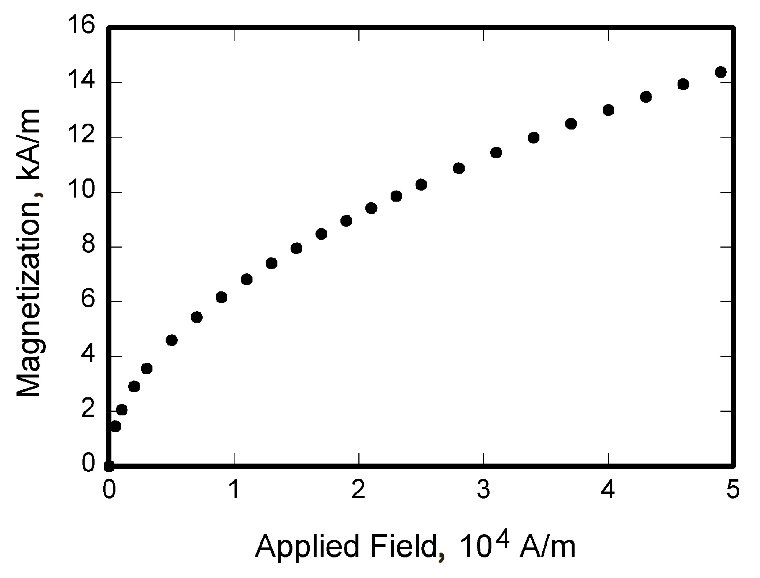
\includegraphics[width=.5\textwidth]{graph}
\caption{Magnetization as a function of applied fields.}
\end{figure}

Line drawings must be clear and sharp. Make sure that all lines and graph points are dark and distinct and that lettering is legible. Keep the lettering size and style uniform both within each figure and throughout all of your illustrations, no smaller than 8- to 10-point type for artwork that is sized to fit the column width (3\,\textonequarter{} in.)~or the full-page width (7\,in.). Place figure captions below each figure, and limit main caption length to 20--25 words. If your figure has multiple parts, include the labels “a),” “b),” etc., below and to the left of each part, above the figure caption. Please verify that the figures and tables you mention in the text actually exist. When citing a figure in the text, use the abbreviation “Fig.” except at the beginning of a sentence. Do not abbreviate “Table.” Number each different type of illustration (i.e., figures and tables) sequentially with relation to other illustrations of the same type.

Figures that are slightly wider than the column width will be reduced in size to fit, so ensure that labels will remain legible (no smaller than 8 to 10 points) after reduction to column width. 

All tables are numbered consecutively and must be cited in the text; give each table a definitive title. Be sure that you have a minimum of two columns (with headings) and two rows to constitute a proper table; otherwise reformat as a displayed list or incorporate the data into the text. Plan tables to fit the column width (3 ¼ in.) or the journal page width (7 in.). Position a double rule at the top and bottom of each table and single rule under the column headings; do not use shading, border lines, or vertical rules between table columns. Position each table in the text close to where it is cited


\subsection{Equations}
Equations are numbered consecutively, with equation numbers in parentheses flush right, as in Eq.~\eqref{sample:equation}. Insert a blank line on either side of the equation. To insert an equation into the \LaTeX{} document, use the \verb|\begin{equation}...\end{equation}| command environment.

A sample equation is included here, formatted using the preceding instructions:

\begin{equation}
\label{sample:equation}
\int^{r_2}_0 F(r,\varphi){\rm d}r\,{\rm d}\varphi = [\sigma r_2/(2\mu_0)]\int^{\infty}_0\exp(-\lambda|z_j-z_i|)\lambda^{-1}J_1 (\lambda r_2)J_0 (\lambda r_i\,\lambda {\rm d}\lambda)
\end{equation}

Be sure that symbols in your equation are defined in the Nomenclature or immediately following the equation. Also define abbreviations and acronyms the first time they are used in the main text. (Very common abbreviations such as AIAA and NASA, do not have to be defined.)

\subsection{General Grammar and Preferred Usage}
Use only one space after periods or colons. Hyphenate complex modifiers: ``zero-field-cooled magnetization.'' Insert a zero before decimal points: ``0.25,'' not ``.25.'' Use ``\si{\centi\meter\squared}'' not ``cc.'' 

A parenthetical statement at the end of a sentence is punctuated outside of the closing parenthesis (like this). (A parenthetical sentence is punctuated within parenthesis.) Use American, not English, spellings (e.g., “color,” not “colour”). The serial comma is preferred: “A, B, and C” instead of “A, B and C.”

Be aware of the different meanings of the homophones “affect” (usually a verb) and “effect” (usually a noun), “complement” and “compliment,” “discreet” and “discrete,” “principal” (e.g., “principal investigator”) and “principle” (e.g., “principle of measurement”). Do not confuse “imply” and “infer.”
\subsection{Footnotes and References}
Footnotes, where they appear, should be placed above the 1'' margin at the bottom of the page. Numbered footnotes are acceptable, but superscript symbols are the preferred AIAA style, in the sequence, *, $\dag$, $\ddag$, \S, \P, **, $\dag\dag$, $\ddag\ddag$, \S\S, etc.

List and number all references at the end of the paper. Corresponding bracketed numbers are used to cite references in the text \cite{vatistas1986reverse}, including citations that are an integral part of the sentence (e.g., ``It is shown in \cite{dornheim1996planetary} that\ldots '') or follow a mathematical expression: ``$A^{2} + B = C$ (Ref.~\cite{terster1997nasa}).'' For multiple citations, separate reference numbers with commas \cite{peyret2012computational,oates1997aerothermodynamics}, or use a dash to show a range \cite{volpe1994techniques,thompsonspacecraft,chi1993fluid,brandis2016nonequi}. Reference citations in the text should be in numerical order. 

In the reference list, give all authors' names; do not use ``et al.''. Papers that have not been published should be cited as ``unpublished''; papers that have been submitted or accepted for publication should be cited as ``submitted for publication.'' Private communications and personal website should appear as footnotes rather than in the reference list.

References should be cited according to the standard publication reference style (for examples, see the ``References'' section of this template). Never edit titles in references to conform to AIAA style of spellings, abbreviations, etc. Names and locations of publishers should be listed; month and year should be included for reports and papers. For papers published in translation journals, please give the English citation first, followed by the original foreign language citation.

\end{document}
